% =====================================================================
%  CHƯƠNG 6. HỆ THỐNG ĐIỀU KHIỂN BÁM NGƯỜI
%  Mã nguồn: follow_drone/ (main.py, follow/*.py, config.yaml)
%  Số đo: runs/control_rate_2026-08-27.md, runs/mavlink_check_2026-08-27.md
% =====================================================================
\chapter{Hệ thống điều khiển máy bay bám theo người}
\label{chap:dieukhien}

Chương này trình bày chương trình máy tính điều khiển máy bay tự động đi theo người, tương ứng nội dung thứ ba của thuyết minh. Chương trình chạy trên Raspberry Pi~5, nhận kết quả phát hiện từ Chương~\ref{chap:trienkhai}, và gửi lệnh vận tốc tới bộ điều khiển bay ArduPilot. Thiết kế tuân theo một nguyên tắc xuyên suốt: phần mềm chỉ \textit{đề xuất} vận tốc trong một chế độ bay mà người lái đã chủ động giao quyền; mọi quyền quyết định chế độ bay thuộc về người lái.

\section{Kiến trúc tổng thể}

\begin{figure}[H]
\centering
\resizebox{\textwidth}{!}{% Kiến trúc tổng thể hệ thống UAV bám người
\begin{tikzpicture}[
  font=\footnotesize, >={Stealth[length=2mm]},
  m/.style={draw=black!60, rounded corners=2pt, align=center, minimum height=11mm, text width=2.6cm, inner sep=2pt, fill=white},
  pi/.style={m, fill=xanh!12},
  hw/.style={m, fill=black!6},
  fc/.style={m, fill=cam!14},
  lb/.style={font=\scriptsize, fill=white, inner sep=1pt}
]
% hàng 1: nhận thức
\node[hw] (cam) at (0,0) {Camera C270\\30 khung/giây};
\node[pi] (det) at (3.6,0) {Phát hiện người\\SteadyDet-N INT8};
\node[hw] (npu) at (3.6,1.9) {NPU Hailo-8L};
\node[pi] (trk) at (7.2,0) {Theo vết\\OC-SORT};
\node[pi] (sel) at (10.8,0) {Chọn \& khoá\\mục tiêu};
% hàng 2: điều khiển
\node[pi] (dist) at (10.8,-2.2) {Ước lượng khoảng cách\\pinhole + Kalman};
\node[pi] (servo) at (7.2,-2.2) {Servo thị giác\\3 bộ PID};
\node[pi] (safe) at (3.6,-2.2) {Lớp an toàn\\giới hạn + thang mất MT};
\node[pi] (mav) at (0,-2.2) {MAVLink client\\30\,Hz, chỉ khi GUIDED};
% hàng 3: phần cứng bay + người
\node[fc] (px) at (0,-4.8) {Pixhawk 6C\\ArduPilot};
\node[hw] (mot) at (3.6,-4.8) {Bộ điều tốc\\+ động cơ};
\node[hw, text width=3.0cm] (web) at (7.2,-4.8) {Bảng giám sát web\\(laptop, điện thoại)};
\node[hw] (rc) at (10.8,-4.8) {Tay điều khiển RC\\(người lái)};

\draw[->] (cam) -- (det);
\draw[<->] (det) -- (npu);
\draw[->] (det) -- (trk);
\draw[->] (trk) -- (sel);
\draw[->] (sel) -- (dist);
\draw[->] (dist) -- (servo);
\draw[->] (servo) -- (safe);
\draw[->] (safe) -- (mav);
\draw[<->] (mav) -- node[lb,right]{USB, MAVLink v2} (px);
\draw[->] (px) -- (mot);
\draw[->, dashed] (servo.south) ++(-0.4,0) -- ++(0,-1.45) node[lb,pos=0.5,left]{hình + trạng thái} ;
\draw[<-, dashed] ($(web.north)+(0.4,0)$) -- node[lb,right]{nút đổi mục tiêu} ($(servo.south)+(0.4,0)$);
\draw[->, thick, draw=cam] (rc.south) -- ++(0,-0.55) -| node[lb,pos=0.25,below]{gạt công tắc chế độ bay (luôn ưu tiên)} (px.south);

\begin{scope}[on background layer]
\node[draw=black!45, dashed, rounded corners=4pt, inner sep=7pt, fit=(det)(npu)(trk)(sel)(dist)(servo)(safe)(mav),
      label={[font=\footnotesize\bfseries, anchor=north east]north east:{Raspberry Pi 5 — chương trình \texttt{main.py}}}] {};
\end{scope}
\end{tikzpicture}
}
\caption{Kiến trúc tổng thể hệ thống. Toàn bộ khối xử lý nằm trên Raspberry Pi~5; bảng giám sát chỉ đọc (trừ nút đổi mục tiêu); tay điều khiển RC luôn có quyền ưu tiên cao nhất}
\label{fig:hethong}
\end{figure}

Hình~\ref{fig:hethong} mô tả luồng dữ liệu. Chương trình \texttt{main.py} gồm các mô-đun: \texttt{camera.py} (luồng đọc camera riêng, luôn trả khung mới nhất), \texttt{detector\_hailo.py} (suy luận trên NPU và hậu xử lý), \texttt{ocsort.py} (theo vết), \texttt{target\_selector.py} (chọn và khoá mục tiêu), \texttt{distance.py} (ước lượng khoảng cách), \texttt{visual\_servo.py} và \texttt{pid.py} (tính vận tốc), \texttt{safety.py} (lớp an toàn), \texttt{mavlink\_client.py} (giao tiếp với bộ điều khiển bay) và \texttt{dashboard.py} (bảng giám sát web). Mọi tham số được đặt trong một tệp cấu hình \texttt{config.yaml} duy nhất.

Bộ điều khiển bay Pixhawk~6C nối với Pi qua cổng USB. Vì cổng nối tiếp này chỉ cho phép một tiến trình mở, đề tài viết thêm công cụ \texttt{mavmux.py}: một tiến trình giữ cổng USB và phát lại nguyên từng byte ra hai cổng UDP nội bộ (14550 cho vòng bám, 14551 dự phòng cho trạm mặt đất). Kiểm tra với hai chương trình đồng thời cho thấy mỗi bên nhận khoảng 100 gói tin/giây với đầy đủ thông tin trạng thái.

\section{Vòng lặp điều khiển}

Vòng lặp chính chạy với chu kỳ 33,3\,ms (30\,Hz) và thực hiện tuần tự mười bước như Hình~\ref{fig:vongdieukhien}.

\begin{figure}[H]
\centering
\resizebox{!}{0.62\textheight}{% Lưu đồ một vòng lặp điều khiển 30 Hz
\begin{tikzpicture}[
  font=\footnotesize, >={Stealth[length=2mm]},
  st/.style={draw=black!60, rounded corners=2pt, align=center, minimum height=8mm, text width=5.2cm, inner sep=2pt, fill=white},
  sm/.style={st, text width=3.6cm},
  io/.style={st, fill=xanh!12},
  dc/.style={diamond, draw=black!60, aspect=2.8, align=center, inner sep=0pt, fill=cam!10, font=\scriptsize, text width=2.4cm},
  tm/.style={st, rounded corners=9pt, fill=black!8}
]
\node[tm] (s) at (0,0) {Bắt đầu vòng lặp (chu kỳ 33,3\,ms)};
\node[io] (a) at (0,-1.1) {1. Lấy khung mới nhất từ camera};
\node[st] (b) at (0,-2.2) {2. Phát hiện người trên NPU (ngưỡng 0,25; NMS)};
\node[st] (c) at (0,-3.3) {3. Cập nhật bộ theo vết OC-SORT};
\node[st] (d) at (0,-4.4) {4. Chọn/khoá mục tiêu (xử lý nút đổi mục tiêu)};
\node[io] (e) at (0,-5.5) {5. Đọc trạng thái máy bay qua MAVLink};
\node[dc] (f) at (0,-6.9) {Có mục tiêu?};
\node[sm] (g) at (-3.4,-8.4) {6. Khoảng cách pinhole + Kalman $\rightarrow$ 3 PID $\rightarrow$ giới hạn an toàn};
\node[sm] (h) at (3.4,-8.4) {Đặt lại các bộ PID};
\node[st] (i) at (0,-9.9) {7. Cập nhật thang mất mục tiêu\\8. Kiểm tra sức khoẻ hệ thống};
\node[dc] (j) at (0,-11.5) {Đang ở GUIDED?};
\node[sm, fill=xanh!12] (k) at (-3.4,-13.0) {9. Gửi vận tốc: FOLLOW / COAST ($\times0{,}5$) / HOVER (0)};
\node[sm] (l) at (3.4,-13.0) {Không gửi lệnh (người lái đang giữ quyền)};
\node[st] (m) at (0,-14.5) {10. Ghi log CSV, cập nhật bảng giám sát};
\foreach \x/\y in {s/a,a/b,b/c,c/d,d/e,e/f,i/j} \draw[->] (\x) -- (\y);
\draw[->] (f.west) -| node[pos=0.25,above,font=\scriptsize]{có} (g.north);
\draw[->] (f.east) -| node[pos=0.25,above,font=\scriptsize]{không} (h.north);
\draw[->] (g.south) |- (i.west);
\draw[->] (h.south) |- (i.east);
\draw[->] (j.west) -| node[pos=0.25,above,font=\scriptsize]{có} (k.north);
\draw[->] (j.east) -| node[pos=0.25,above,font=\scriptsize]{không} (l.north);
\draw[->] (k.south) |- (m.west);
\draw[->] (l.south) |- (m.east);
\draw[->] (m.south) -- ++(0,-0.4) -- ++(6.0,0) |- (s.east);
\end{tikzpicture}
}
\caption{Lưu đồ một vòng lặp điều khiển 30\,Hz trong \texttt{main.py}}
\label{fig:vongdieukhien}
\end{figure}

Có ba điểm đáng chú ý trong lưu đồ. \textit{Thứ nhất}, khi không có mục tiêu, các bộ PID được đặt lại để thành phần tích phân không tích luỹ sai số cũ. \textit{Thứ hai}, lệnh vận tốc chỉ được gửi khi máy bay đang ở chế độ GUIDED; ở mọi chế độ khác chương trình im lặng và in một dòng thông báo. \textit{Thứ ba}, bước ghi nhật ký và cập nhật bảng giám sát dùng lại chính khung hình và kết quả phát hiện của vòng lặp, không tốn thêm lượt suy luận nào; điều này bắt buộc vì NPU Hailo chỉ cho phép một tiến trình sử dụng.

\section{Theo vết đa đối tượng}

Kết quả phát hiện ở từng khung độc lập với nhau, trong khi bộ điều khiển cần biết người \textit{nào} đang được bám qua thời gian. Đề tài dùng OC-SORT~\cite{cao2023ocsort} vì ba lý do: không cần mạng trích đặc trưng ngoại hình nên chạy nhẹ trên CPU; xử lý tốt trường hợp mất phát hiện vài khung nhờ hiệu chỉnh dựa trên quan sát; và có kết quả tốt trên các benchmark theo vết người. Mỗi đối tượng được biểu diễn bằng một bộ lọc Kalman với trạng thái gồm tâm hộp, diện tích, tỷ lệ khung hình và vận tốc tương ứng. Phát hiện mới được ghép với dự đoán bằng thuật toán Hungary trên ma trận IoU.

\begin{table}[H]
\centering
\caption{Tham số bộ theo vết OC-SORT}
\label{tab:ocsort}
\small
\renewcommand{\arraystretch}{1.15}
\begin{tabularx}{\textwidth}{@{}lc>{\raggedright\arraybackslash}X@{}}
\toprule
\textbf{Tham số} & \textbf{Giá trị} & \textbf{Ý nghĩa và lý do chọn}\\
\midrule
\texttt{max\_age} & 45 khung & Giữ vết sống 1,5\,s khi mất phát hiện. Giá trị ban đầu 90 (3\,s) quá dài: bám theo dự đoán 3 giây thì người đã kịp đổi hướng\\
\texttt{min\_hits} & 3 & Cần 3 lần phát hiện liên tiếp mới xác nhận vết, loại bỏ hộp sai thoáng qua\\
\texttt{iou\_threshold} & 0,3 & Ngưỡng IoU tối thiểu để ghép phát hiện với vết\\
\texttt{delta\_t} & 3 & Số khung nhìn lại để ước lượng hướng chuyển động\\
\bottomrule
\end{tabularx}
\end{table}

Trước khi đưa vào bộ theo vết, phát hiện được lọc thêm hai điều kiện đơn giản: bỏ các hộp có diện tích dưới 200 điểm ảnh vuông và các hộp có tỷ lệ cạnh lớn hơn 6, vì người ở độ cao 3--6\,m luôn lớn hơn và có hình dạng hợp lý hơn thế.

\section{Chọn và khoá mục tiêu}

Khi có nhiều người trong khung hình, hệ thống phải chọn một người và bám ổn định người đó. Chiến lược mặc định chọn hộp có diện tích lớn nhất (thường là người gần nhất) ở lần đầu, rồi \textbf{khoá vào mã định danh} của vết đó; sau khi khoá, hệ thống bám đúng người này kể cả khi có người khác xuất hiện gần hơn.

Một khó khăn thực tế là OC-SORT cấp mã định danh \textit{mới} cho người rời khung rồi quay lại, vì nó không có cơ chế nhận dạng lại theo ngoại hình. Nếu không xử lý, sau khi mất mục tiêu, hệ thống có thể khoá nhầm vào một người lạ đứng gần hơn. Đề tài giải quyết bằng một cơ chế liên tục không gian đơn giản:
\begin{enumerate}
\item Khi mục tiêu biến mất, khoá được giữ thêm $3$\,s (\texttt{lost\_grace\_s}), bằng đúng pha máy bay còn bám theo dự đoán.
\item Sau khi nhả khoá, trong $5$\,s tiếp theo (\texttt{reacquire\_s}) hệ thống \textit{chỉ} chấp nhận một vết có tâm cách vị trí cuối của mục tiêu cũ không quá 25\% đường chéo khung hình và diện tích chênh không quá 2 lần. Người cũ quay lại chỗ cũ, dù mang mã mới, được bám lại ngay; người lạ không bị ``vồ'' nhầm.
\item Hết cửa sổ tìm lại, hệ thống mới chọn mục tiêu mới theo chiến lược (có thể tắt để chờ người vận hành bằng \texttt{auto\_relock: false}).
\end{enumerate}
Hai ngưỡng ở bước 2 được đặt chặt có chủ ý: thà không nhận ra còn hơn bám nhầm người. Cơ chế này đúng khi người quay lại gần chỗ cũ và có thể sai khi hai người đổi chỗ cho nhau, vì vậy bảng giám sát có nút \textbf{Đổi mục tiêu} cho người vận hành bỏ khoá và chọn lại ngay lập tức. Toàn bộ các tình huống trên được kiểm tra bằng bộ kiểm thử tự động \texttt{test\_target\_selector.py} gồm 14 phép kiểm tra (Chương~\ref{chap:tichhop}).

\begin{table}[H]
\centering
\caption{Diễn biến hành vi khi mất mục tiêu (tính từ lần cuối nhìn thấy)}
\label{tab:matmuctieu}
\small
\renewcommand{\arraystretch}{1.15}
\begin{tabularx}{\textwidth}{@{}l>{\raggedright\arraybackslash}X>{\raggedright\arraybackslash}X@{}}
\toprule
\textbf{Thời gian} & \textbf{Bám ai (bộ chọn mục tiêu)} & \textbf{Máy bay làm gì (lớp an toàn)}\\
\midrule
0 -- 1,5\,s & OC-SORT giữ vết bằng dự đoán Kalman & Tiếp tục bám\\
1,5 -- 4,5\,s & Vẫn giữ khoá mục tiêu & COAST: vận tốc giảm một nửa (từ 0 tới 3\,s mất mục tiêu)\\
4,5 -- 9,5\,s & Chỉ tìm lại đúng người cũ & HOVER: vận tốc bằng 0, đứng yên\\
sau 9,5\,s & Cho phép chọn người khác & HOVER cho tới khi thấy lại mục tiêu hoặc người lái lấy lại quyền\\
\bottomrule
\end{tabularx}
\end{table}

\section{Ước lượng khoảng cách}

Khoảng cách tới người được ước lượng từ chiều cao bounding box theo mô hình lỗ kim, phương trình~(\ref{eq:distance}), với chiều cao người giả định $H_r = 1{,}7$\,m. Tệp cấu hình hiện đặt tiêu cự $f_x = f_y = 700$ điểm ảnh và tâm ảnh $(320, 240)$ cho độ phân giải $640\times480$; hệ thống kèm công cụ \texttt{calibrate\_camera.py} để hiệu chuẩn lại bằng bàn cờ theo phương pháp của Zhang~\cite{zhang2000calibration}. Độ phân giải camera được giữ ở $640\times480$ vì hai lý do: các tham số nội của camera gắn với độ phân giải này (chuyển sang 16:9 làm thay đổi cả góc nhìn chứ không chỉ tỷ lệ), và mô hình vốn đưa ảnh về 640 điểm ảnh nên độ phân giải cao hơn không thêm điểm ảnh nào trên người mà chỉ tốn CPU giải nén.

Kết quả đo được loại bỏ khi hộp thấp hơn 20 điểm ảnh hoặc khoảng cách nằm ngoài khoảng 0,5--30\,m. Vì sai số tăng theo bình phương khoảng cách, phương sai đo được mô hình hoá là $\sigma^2 = \max\big(0{,}1,\ (2d^2/f_y)^2\big)$, ứng với sai số chiều cao hộp khoảng 2 điểm ảnh. Giá trị đo được làm mượt bằng bộ lọc Kalman một chiều với trạng thái $[d,\ \dot d]^\top$, mô hình vận tốc không đổi; phương sai đo thay đổi theo từng lần đo nên các phép đo ở xa (kém tin cậy) tự động được tin ít hơn.

\section{Servo thị giác và bộ điều khiển PID}

Đề tài dùng cách tiếp cận servo thị giác lai~\cite{chaumette2006visual}: kênh quay hướng dùng sai số trực tiếp trên ảnh, kênh tiến lùi dùng khoảng cách ước lượng, kênh độ cao dùng độ cao đo từ bộ điều khiển bay. Ba bộ điều khiển PID độc lập theo phương trình~(\ref{eq:pid}) sinh ra vận tốc trong hệ toạ độ thân máy bay; vận tốc ngang bằng 0 vì chuyển động sang ngang được thực hiện bằng cách quay hướng.

\begin{itemize}
\item \textbf{Kênh tiến lùi:} sai số là khoảng cách đã làm mượt trừ khoảng cách đặt 5\,m. Người ở xa hơn 5\,m thì máy bay tiến tới, gần hơn thì lùi lại. Khi không có khoảng cách tin cậy, vận tốc tiến bằng 0.
\item \textbf{Kênh quay hướng:} sai số góc $e_\psi = (u_c - W/2)/f_x$ (radian), với $u_c$ là hoành độ tâm hộp và $W$ là bề rộng ảnh. Người lệch phải thì máy bay quay phải. Kênh này không dùng thành phần tích phân: sai số góc tự về 0 khi máy bay quay tới, còn tích phân chỉ tích luỹ rồi gây vọt lố mỗi khi mục tiêu ra khỏi khung.
\item \textbf{Kênh độ cao:} giữ độ cao 5\,m so với mặt đất; đầu ra được đổi dấu khi gửi vì trục $z$ của hệ NED hướng xuống.
\end{itemize}

\begin{table}[H]
\centering
\caption{Tham số ba bộ điều khiển PID}
\label{tab:pid}
\small
\renewcommand{\arraystretch}{1.15}
\begin{tabular}{@{}lcccccc@{}}
\toprule
\textbf{Kênh} & \textbf{Giá trị đặt} & \textbf{$K_p$} & \textbf{$K_i$} & \textbf{$K_d$} & \textbf{Giới hạn đầu ra} & \textbf{Giới hạn tích phân}\\
\midrule
Tiến lùi & 5,0\,m & 0,5 & 0,05 & 0,1 & $\pm$3,0\,m/s & $\pm$2,0\\
Quay hướng & 0\,rad & 2,0 & 0 & 0,3 & $\pm$1,5\,rad/s & --\\
Độ cao & 5,0\,m & 0,8 & 0,1 & 0,2 & $\pm$2,0\,m/s & $\pm$1,0\\
\bottomrule
\end{tabular}
\end{table}

Bước thời gian được đo thực tế giữa hai lần gọi thay vì giả định cố định. Nếu khoảng cách giữa hai lần gọi vượt 1\,s (ví dụ sau khi mất mục tiêu lâu), bộ điều khiển tự đặt lại để tránh thành phần vi phân và tích phân nhận giá trị bất thường. Vận tốc trong hệ thân được chuyển sang hệ NED bằng góc hướng hiện tại $\psi$ của máy bay:
\begin{equation}
v_N = v_x \cos\psi - v_y \sin\psi, \qquad v_E = v_x \sin\psi + v_y \cos\psi,
\end{equation}
rồi gửi bằng thông điệp \texttt{SET\_POSITION\_TARGET\_LOCAL\_NED} với mặt nạ chỉ dùng ba thành phần vận tốc và tốc độ quay hướng.

\section{Lớp an toàn}
\label{sec:antoan}

An toàn được thiết kế nhiều lớp, mỗi lớp độc lập với các lớp còn lại.

\textbf{Giới hạn lệnh.} Vận tốc ngang bị chặn $\pm$5\,m/s, vận tốc đứng $\pm$2\,m/s, tốc độ quay hướng $\pm$1,0\,rad/s (57\,°/s, thấp hơn giới hạn 60\,°/s của bộ điều khiển bay để lệnh không bị cắt). Khi người ở gần hơn 3\,m, máy bay bị buộc lùi với vận tốc ít nhất 0,5\,m/s; khi xa hơn 15\,m, vận tốc tiến bị giới hạn 1\,m/s vì phát hiện ở xa kém tin cậy. Máy bay không được hạ thấp hơn 2\,m hay lên cao quá 25\,m so với mặt đất.

\textbf{Kiểm tra trước khi cất cánh.} Chương trình chỉ cất cánh khi GPS có định vị 3D với HDOP không quá 2,0, điện áp pin không dưới 14,8\,V (3,7\,V mỗi cell với pin 4S) và gói \texttt{HEARTBEAT} mới nhất cách không quá 2\,s.

\textbf{Kiểm tra trong khi bay.} Mỗi vòng lặp kiểm tra: mất \texttt{HEARTBEAT} quá 3\,s, mất định vị GPS, pin dưới 14,0\,V, độ cao vượt 1,5 lần giới hạn. Khi một điều kiện bị vi phạm, chương trình \textbf{ngừng gửi lệnh và thoát vòng bám, nhưng không đổi chế độ bay}. Bộ điều khiển bay tự dừng máy bay sau thời gian \texttt{GUID\_TIMEOUT} = 1\,s, còn người lái lấy lại quyền bằng công tắc chế độ.

\textbf{Thang mất mục tiêu.} Hình~\ref{fig:antoan} mô tả máy trạng thái. Khi mất mục tiêu dưới 3\,s (COAST), máy bay tiếp tục theo lệnh tính từ dự đoán với vận tốc giảm một nửa; sau 3\,s (HOVER), vận tốc bằng 0 và máy bay đứng yên cho tới khi thấy lại mục tiêu hoặc người lái chuyển chế độ. Thang \textit{không} leo thang sang LOITER hay RTL: chế độ RTL của ArduPilot trước tiên leo lên độ cao an toàn \texttt{RTL\_ALT} (mặc định 15\,m), một hành động bất ngờ với người lái nếu phần mềm tự kích hoạt, nên quyết định chuyển chế độ được dành cho người lái.

\begin{figure}[H]
\centering
\resizebox{0.85\textwidth}{!}{% Máy trạng thái thang mất mục tiêu
\begin{tikzpicture}[
  font=\footnotesize, >={Stealth[length=2mm]},
  s/.style={circle, draw=black!60, align=center, minimum size=19mm, inner sep=1pt, fill=white},
]
\node[s, fill=xanh!15] (F) {FOLLOW\\\scriptsize bám theo};
\node[s, fill=cam!12, right=3.2cm of F] (C) {COAST\\\scriptsize vận tốc $\times0{,}5$};
\node[s, fill=black!8, right=3.2cm of C] (H) {HOVER\\\scriptsize vận tốc 0};
\draw[->] (F) to[bend left=18] node[above,font=\scriptsize,align=center]{mất mục tiêu} (C);
\draw[->] (C) to[bend left=18] node[below,font=\scriptsize]{thấy lại} (F);
\draw[->] (C) -- node[above,font=\scriptsize,align=center]{mất $\ge$ 3\,s} (H);
\draw[->] (H) to[bend left=35] node[below,font=\scriptsize]{thấy lại mục tiêu} (F);
\draw[->] (H) edge[loop right] node[right,font=\scriptsize,align=left]{đứng yên đến khi\\người lái gạt\\công tắc chế độ} (H);
\end{tikzpicture}
}
\caption{Máy trạng thái của thang mất mục tiêu; phần mềm không bao giờ tự đổi chế độ bay}
\label{fig:antoan}
\end{figure}

\textbf{Người lái luôn giữ quyền.} Phần mềm chỉ gọi lệnh đổi chế độ bay ở đúng một chỗ: chuỗi cất cánh tự động khi người vận hành chủ động chạy chương trình ở chế độ bay thật. Mọi lệnh vận tốc chỉ được gửi khi máy bay đang ở GUIDED; gạt công tắc sang LOITER hay STABILIZE là phần mềm im lặng ngay lập tức. Nhấn Ctrl+C gửi vận tốc 0 rồi buông quyền, không tự quay về. Nguyên tắc này được khoá bằng bộ kiểm thử \texttt{test\_safety\_no\_mode\_change.py}, trong đó có phép kiểm tra quét mã nguồn \texttt{safety.py} để đảm bảo không còn lời gọi đổi chế độ nào.

\textbf{Tham số trên bộ điều khiển bay.} Khi kết nối lần đầu với Pixhawk~6C (ArduPilot Copter 4.7.0), nhóm tải đủ 1.038 tham số và phát hiện năm cấu hình không an toàn cần sửa trước khi bay tự động: bỏ qua toàn bộ kiểm tra trước khi arm (\texttt{ARMING\_SKIPCHK} = $-1$), ngưỡng pin yếu và pin nguy kịch bị đặt ngược nhau (10\,V và 14\,V), không có hành động khi pin yếu, không có bảo vệ khi mất máy tính đồng hành (\texttt{FS\_GCS\_ENABLE} = 0), và hàng rào địa lý đã cấu hình nhưng đang tắt. Bảng tham số khuyến nghị được trình bày ở Phụ lục~A. Một lưu ý quan trọng là ArduPilot 4.7 đã đổi tên và đơn vị nhiều tham số (ví dụ \texttt{WPNAV\_SPEED} tính bằng cm/s thành \texttt{WP\_SPD} tính bằng m/s); chép giá trị từ tài liệu cho phiên bản cũ sẽ sai tới 100 lần.

\section{Giao tiếp MAVLink và lựa chọn nhịp gửi lệnh}

\subsection{Kiểm tra liên lạc}

Kết nối được kiểm tra trực tiếp trên máy bay (không phải mô phỏng): Pixhawk~6C chạy ArduPilot Copter 4.7.0, MAVLink v2, nhận 94--100 gói tin/giây với 0 lỗi truyền. Các thông điệp cần cho bảng giám sát đều về đủ nhịp: \texttt{ATTITUDE}, \texttt{VFR\_HUD}, \texttt{GLOBAL\_POSITION\_INT} ở 10\,Hz; \texttt{SYS\_STATUS}, \texttt{GPS\_RAW\_INT} ở 5\,Hz; \texttt{VIBRATION}, \texttt{EKF\_STATUS\_REPORT}, \texttt{BATTERY\_STATUS} ở 3,1\,Hz. Mọi cảm biến ở trạng thái tốt, các phương sai EKF3 dưới 0,01 và mức rung nền 0,01--0,07\,m/s² khi chưa quay động cơ. Quá trình kiểm tra cũng phát hiện hai lỗi trong mã của nhóm: chương trình đọc trạng thái gửi yêu cầu nhịp thông điệp \textit{chậm hơn} nhịp mà ArduPilot đang tự phát (làm giảm \texttt{VFR\_HUD} từ 10 xuống 5\,Hz), và bảng bit trạng thái cảm biến gõ tay bị lệch khiến trạng thái sẵn sàng arm không bao giờ đọc được. Cả hai đã được sửa: chỉ yêu cầu những thông điệp chưa nhận được sau 3 giây lắng nghe, và sinh bảng bit trực tiếp từ định nghĩa của thư viện pymavlink.

\subsection{Chọn nhịp gửi lệnh 30\,Hz}

Nhịp gửi lệnh được chọn dựa trên số đo. Khứ hồi một lệnh từ Pi tới máy bay và nhận xác nhận có trung vị 4,75\,ms, p95 6,24\,ms, p99 7,73\,ms (120 mẫu), tức một chiều khoảng 2,4\,ms; gửi ở 50\,Hz không mất gói nào (200/200). Độ trễ từ lúc ánh sáng vào cảm biến tới lúc lệnh tới bộ điều khiển bay gồm độ trễ phát hiện (32,0\,ms), thời gian chờ tới lượt gửi và thời gian truyền (Bảng~\ref{tab:nhiplenh}, Hình~\ref{fig:nhiplenh}).

\begin{table}[H]
\centering
\caption{Ngân sách độ trễ từ ảnh tới lệnh theo nhịp gửi (ms)}
\label{tab:nhiplenh}
\small
\renewcommand{\arraystretch}{1.15}
\begin{tabular}{@{}lccccc@{}}
\toprule
\textbf{Nhịp gửi} & \textbf{Phát hiện} & \textbf{Chờ (TB / xấu nhất)} & \textbf{Truyền} & \textbf{Tổng TB} & \textbf{Tổng xấu nhất}\\
\midrule
10\,Hz & 32,0 & 50,0 / 100,0 & 2,4 & 84,4 & 138,4\\
20\,Hz & 32,0 & 25,0 / 50,0 & 2,4 & 59,4 & 88,4\\
\textbf{30\,Hz} & 32,0 & \textbf{16,7 / 33,3} & 2,4 & \textbf{51,1} & \textbf{71,7}\\
50\,Hz & 32,0 & 10,0 / 20,0 & 2,4 & 44,4 & 58,4\\
\bottomrule
\end{tabular}
\end{table}

\begin{figure}[H]
\centering
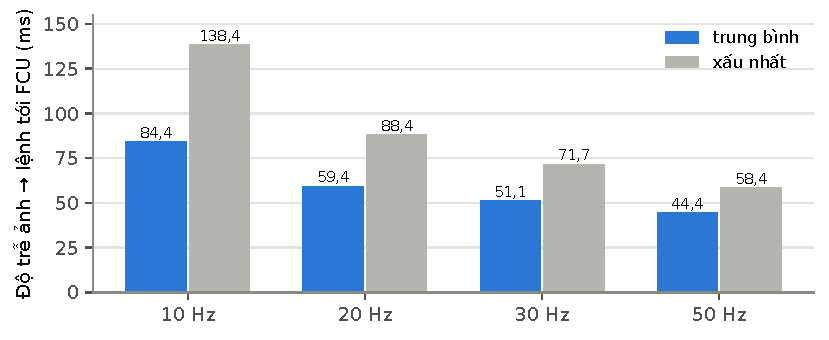
\includegraphics[width=0.9\textwidth]{nhip_lenh.pdf}
\caption{Độ trễ từ ảnh tới lệnh theo nhịp gửi}
\label{fig:nhiplenh}
\end{figure}

Ở 10\,Hz, mỗi phát hiện phải chờ trung bình 50\,ms mới được gửi đi: thêm 50\,ms trễ mà không đổi lấy lợi ích gì. Với người đi bộ 1,5\,m/s, 50\,ms tương ứng 7,5\,cm sai lệch, và trong vòng kín nó tích luỹ thành vọt lố. Ở 50\,Hz, vì bộ phát hiện chỉ sinh thông tin mới 30 lần mỗi giây, 20 trong 50 lệnh không mang phát hiện mới nào, trong khi chỉ lợi thêm 6,7\,ms. \textbf{Nhịp 30\,Hz khớp một-một với nhịp của bộ phát hiện}: mỗi lệnh mang đúng một phát hiện mới. Băng thông tương ứng khoảng 2\,KB/s, không đáng kể với đường USB. Nhịp này cũng nằm trong vùng hoạt động tốt mà các lập trình viên ArduPilot khuyến nghị cho chế độ GUIDED (trên 10\,Hz)~\cite{ardupilot}. Kèm theo đó, thời gian chờ lệnh của phần mềm và \texttt{GUID\_TIMEOUT} của máy bay được hạ từ 3\,s xuống 1\,s: ở 30\,Hz, 3\,s tương đương 90 lệnh bị mất trước khi máy bay chịu dừng.

\section{Bảng giám sát và ghi nhật ký}

Bảng giám sát là một trang web do chính \texttt{main.py} phục vụ ở cổng 8080, mở được trên laptop hoặc điện thoại cùng mạng WiFi mà không cần màn hình gắn vào Pi. Trang hiển thị video có vẽ hộp và mục tiêu đang khoá, chế độ bay, trạng thái arm, độ cao, pin, GPS, tư thế, mức rung thật ba trục, trạng thái vòng bám (FOLLOW/COAST/HOVER), khoảng cách ước lượng, bốn thành phần vận tốc đang gửi, độ trễ từng chặng, nhiệt độ SoC và trạng thái giảm xung nhiệt. Thao tác duy nhất trang cho phép là nút \textbf{Đổi mục tiêu}; trang không thể arm, đổi chế độ hay gửi vận tốc.

Mỗi vòng lặp ghi một dòng nhật ký CSV gồm thời gian, trạng thái an toàn, chế độ bay, vị trí và vận tốc máy bay, độ cao, pin, GPS, mã mục tiêu, bounding box, khoảng cách thô và đã làm mượt, lệnh vận tốc, cùng \textbf{mức rung ba trục, số lần bão hoà cảm biến gia tốc, số phát hiện và điểm tin cậy cao nhất}. Việc đặt mức rung đo thật và chất lượng phát hiện trên cùng một dòng, cùng một dấu thời gian là cơ sở để đối chiếu mô hình rung mô phỏng của Chương~\ref{chap:dulieu} với rung thật trong các chuyến bay tiếp theo.

\section{Kết luận chương}

Chương trình điều khiển bám người đã được xây dựng hoàn chỉnh: theo vết OC-SORT, khoá mục tiêu có cơ chế tìm lại người cũ, ước lượng khoảng cách pinhole có bộ lọc Kalman, ba bộ PID trong cấu trúc servo thị giác lai, lớp an toàn nhiều tầng với nguyên tắc người lái luôn giữ quyền chế độ bay, giao tiếp MAVLink 30\,Hz với độ trễ và băng thông được đo kiểm, bảng giám sát web và nhật ký bay có dữ liệu rung thật. Mọi tham số quan trọng đều được chọn dựa trên số đo và được ghi lại lý do trong tệp cấu hình.
